\documentclass[11pt]{article}
\usepackage{certmachine}
\usepackage{graphicx}
%% generated by tools/paper-numbers/jacobian-counterexamples.js from certs/keller-certificate.json, certs/polymaps-ledger.json, corpus/polymaps and corpus/sources/PINS.json, with the keller battery, the polymaps battery, tools/verify_keller.py and the fiber family run live — do not edit (git 054078d19462)
\newcommand{\RepoCommit}{054078d19462}
\newcommand{\CertGit}{1d2b452}
\newcommand{\CertSha}{9ee1ff71a81a}
\newcommand{\NCerts}{11}
\newcommand{\NTranscribed}{3}
\newcommand{\NReconstructed}{5}
\newcommand{\NGenerated}{3}
\newcommand{\NPublished}{8}
\newcommand{\NDistinctMaps}{10}
\newcommand{\PaddedN}{8}
\newcommand{\NPinned}{8}
\newcommand{\PinFiles}{\texttt{gallagher2026.pdf} and \texttt{mengyang2026.pdf}}
\newcommand{\NPinFiles}{2}
\newcommand{\MengYangSha}{090c1735997c}
\newcommand{\GallagherSha}{1782eefa569a}
\newcommand{\DetList}{$-2$, $128$, $1$, $-1$}
\newcommand{\DimList}{3, 5, 8}
\newcommand{\TotalWitnessEvals}{24}
\newcommand{\AlpogeDet}{-2}
\newcommand{\AlpogeDegs}{7, 6, 4}
\newcommand{\AlpogeTerms}{7, 6, 3}
\newcommand{\AlpogePoints}{$(0,\, 0,\, -\tfrac{1}{4})$, $(1,\, -\tfrac{3}{2},\, \tfrac{13}{2})$, $(-1,\, \tfrac{3}{2},\, \tfrac{13}{2})$}
\newcommand{\AlpogeImage}{$(-\tfrac{1}{4},\, 0,\, 0)$}
\newcommand{\AlpogeSource}{Alp\"oge 2026-07-19}
\newcommand{\HessDet}{128}
\newcommand{\HessN}{5}
\newcommand{\HessGradDegs}{13, 13, 13, 12, 10}
\newcommand{\HessPoints}{$(1,\, -\tfrac{3}{2},\, 0,\, 0,\, 0)$ and $(-1,\, \tfrac{3}{2},\, 0,\, 0,\, 0)$}
\newcommand{\HessImage}{$(0,\, 0,\, -\tfrac{1}{2},\, 0,\, 0)$}
\newcommand{\PsiDegree}{14}
\newcommand{\PsiMonomials}{42}
\newcommand{\GenDegrees}{3, 4, 5}
\newcommand{\GenGeomDegrees}{4, 5, 6}
\newcommand{\GenGZero}{2}
\newcommand{\GenB}{-1}
\newcommand{\GalDets}{$1$ and $-1$}
\newcommand{\GalGeomDegrees}{3, 4, 5, 6, 4}
\newcommand{\VerEntries}{11}
\newcommand{\VerFails}{0}
\newcommand{\VerPins}{15}
\newcommand{\TotalJacMonos}{1{,}403}
\newcommand{\MaxJacMonos}{339}
\newcommand{\MinJacMonos}{33}
\newcommand{\HessJacMonos}{339}
\newcommand{\BatPass}{32}
\newcommand{\BatReds}{9}
\newcommand{\CalCurve}{[4, -3]}
\newcommand{\AutoStarts}{400}
\newcommand{\DoublingDet}{-4}
\newcommand{\DoublingPhiMonos}{16}
\newcommand{\DoublingHessMonos}{126}
\newcommand{\FibCells}{9}
\newcommand{\FibHits}{7}
\newcommand{\FibRejects}{1}
\newcommand{\FibRefused}{1}
\newcommand{\FibExceeded}{3}
\newcommand{\FibStarts}{400}
\newcommand{\OwnTarget}{$(0,\, 1,\, 0)$}
\newcommand{\FibFailedCells}{\texttt{gallagher-d4} and \texttt{sweep-d5}}
\newcommand{\FibExceededCells}{\texttt{sweep-d3}, \texttt{gallagher-d2}, \texttt{gallagher-d3}}
\newcommand{\FiberRows}{\texttt{alpoge} & the announced map & $(-\tfrac{1}{4},\, 0,\, 0)$ & own collision image & 3 & 3 & $\ge$ 3 preimages, certified \\
\texttt{alpoge-own-target} & the announced map & $(0,\, 1,\, 0)$ & chosen here & 2 & 3 & $\ge$ 3 preimages, certified \\
\texttt{sweep-d3} & generated, curve degree 3 & $(-\tfrac{13}{8},\, -2,\, 1)$ & own collision image & 2 & 3 & $\ge$ 3 preimages, certified \\
\texttt{sweep-d4} & generated, curve degree 4 & $(-\tfrac{13}{5},\, -\tfrac{16}{5},\, 1)$ & own collision image & 2 & 2 & $\ge$ 2 preimages, certified \\
\texttt{sweep-d5} & generated, curve degree 5 & $(-\tfrac{61}{12},\, -\tfrac{19}{3},\, 1)$ & own collision image & 2 & 0 & no certified box \\
\texttt{gallagher-d2} & Gallagher seed $d=2$ & $(-4,\, -4,\, 1)$ & own collision image & 2 & 3 & $\ge$ 3 preimages, certified \\
\texttt{gallagher-d3} & Gallagher seed $d=3$ & $(-\tfrac{1}{2},\, -\tfrac{1}{2},\, 1)$ & own collision image & 2 & 3 & $\ge$ 3 preimages, certified \\
\texttt{gallagher-d4} & Gallagher seed $d=4$ & $(-\tfrac{11}{10},\, -\tfrac{11}{10},\, 1)$ & own collision image & 2 & 1 & one box: nothing proved \\
\texttt{gallagher-distinct} & Gallagher distinct member & $(0,\, 0,\, 1)$ & own collision image & 2 & 2 & $\ge$ 2 preimages, certified \\}
\newcommand{\CertRows}{\texttt{keller-0} & Alp\"oge 19 July 2026, via \cite{MengYang2026} & components of degree 7, 6, 4 & 3 & $-2$ & 3 & 33 & transcribed \\
\texttt{keller-1} & the same map, identity-padded & the $n=3$ map, stabilised once & 8 & $-2$ & 3 & 38 & transcribed \\
\texttt{keller-2} & this repository & curve $[6, -6, 1]$, geometric degree 4 & 3 & $-2$ & 2 & 78 & generated \\
\texttt{keller-3} & this repository & curve $[\tfrac{52}{5}, -\tfrac{51}{5}, 0, 1]$, geometric degree 5 & 3 & $-2$ & 2 & 141 & generated \\
\texttt{keller-4} & this repository & curve $[20, -19, 0, 0, 1]$, geometric degree 6 & 3 & $-2$ & 2 & 222 & generated \\
\texttt{keller-5} & Meng--Yang \cite{MengYang2026} & gradient of $\Psi$, $\deg\Psi=14$ & 5 & $128$ & 2 & 339 & transcribed \\
\texttt{keller-6} & Gallagher \cite{Gallagher2026} & seed $[2, -3]$, generic fiber 3 & 3 & $1$ & 2 & 33 & rebuilt from seed \\
\texttt{keller-7} & Gallagher \cite{Gallagher2026} & seed $[\tfrac{3}{2}, -\tfrac{3}{2}, -1]$, generic fiber 4 & 3 & $1$ & 2 & 78 & rebuilt from seed \\
\texttt{keller-8} & Gallagher \cite{Gallagher2026} & seed $[\tfrac{17}{10}, -\tfrac{27}{10}, 1, -1]$, generic fiber 5 & 3 & $1$ & 2 & 141 & rebuilt from seed \\
\texttt{keller-9} & Gallagher \cite{Gallagher2026} & seed $[\tfrac{9}{5}, -\tfrac{14}{5}, 0, 1, -1]$, generic fiber 6 & 3 & $1$ & 2 & 222 & rebuilt from seed \\
\texttt{keller-10} & Gallagher \cite{Gallagher2026} & seed $[1, 0, -2]$, generic fiber 4 & 3 & $-1$ & 2 & 78 & rebuilt from seed \\}
\newcommand{\GenRows}{\texttt{keller-2} & $[6, -6, 1]$ & $-4$ & 4 & 12, 11, 4 & 78 & $(-\tfrac{2}{3},\, \tfrac{5}{2},\, \tfrac{183}{8})$, $(\tfrac{2}{11},\, -\tfrac{13}{2},\, \tfrac{297}{8})$ \\
\texttt{keller-3} & $[\tfrac{52}{5}, -\tfrac{51}{5}, 0, 1]$ & $-\tfrac{9}{7}$ & 5 & 17, 16, 4 & 141 & $(-\tfrac{5}{11},\, \tfrac{16}{5},\, \tfrac{25707}{875})$, $(\tfrac{5}{41},\, -\tfrac{46}{5},\, -\tfrac{279907}{875})$ \\
\texttt{keller-4} & $[20, -19, 0, 0, 1]$ & $-\tfrac{13}{7}$ & 6 & 22, 21, 4 & 222 & $(-\tfrac{6}{25},\, \tfrac{31}{6},\, \tfrac{222325}{1512})$, $(\tfrac{6}{101},\, -\tfrac{107}{6},\, -\tfrac{5512277}{1512})$ \\}
\newcommand{\GalRows}{\texttt{keller-6} & $[2, -3]$ & $-\tfrac{3}{2}$ & $1$ & $1$ & 3 & $(-\tfrac{1}{3},\, 4,\, -54)$, $(\tfrac{1}{4},\, -2,\, 36)$ \\
\texttt{keller-7} & $[\tfrac{3}{2}, -\tfrac{3}{2}, -1]$ & $-\tfrac{7}{5}$ & $1$ & $1$ & 4 & $(2,\, \tfrac{1}{2},\, \tfrac{9}{40})$, $(\tfrac{2}{3},\, -\tfrac{5}{2},\, -\tfrac{33}{8})$ \\
\texttt{keller-8} & $[\tfrac{17}{10}, -\tfrac{27}{10}, 1, -1]$ & $-\tfrac{37}{27}$ & $1$ & $1$ & 5 & $(-10,\, \tfrac{11}{10},\, -\tfrac{4367}{27000})$, $(\tfrac{10}{53},\, -\tfrac{63}{10},\, \tfrac{225091}{3000})$ \\
\texttt{keller-9} & $[\tfrac{9}{5}, -\tfrac{14}{5}, 0, 1, -1]$ & $-\tfrac{19}{14}$ & $1$ & $1$ & 6 & $(\tfrac{15}{4},\, \tfrac{11}{15},\, \tfrac{5038}{23625})$, $(\tfrac{15}{28},\, -\tfrac{43}{15},\, -\tfrac{14318}{3375})$ \\
\texttt{keller-10} & $[1, 0, -2]$ & $-\tfrac{4}{3}$ & $-1$ & $-1$ & 4 & $(1,\, 0,\, 0)$, $(-1,\, 0,\, 2)$ \\}
\newcommand{\PolyRows}{8}
\newcommand{\PolyCertified}{7}
\newcommand{\PolyPartial}{1}
\newcommand{\PolyGenerated}{2026-10-05}
\newcommand{\PolySeconds}{90}
\newcommand{\GaoArxiv}{2608.00222v1}
\newcommand{\ChvArxiv}{2608.05392v1}
\newcommand{\GaoTitle}{Counterexamples to the Jacobian conjecture in dimensions greater than two}
\newcommand{\ChvTitle}{The weak Markus--Yamabe conjecture fails in dimension 14}
\newcommand{\GaoTexSha}{c644040df103}
\newcommand{\ChvTexSha}{a5cf5acfa67a}
\newcommand{\GaoPdfSha}{483208235e32}
\newcommand{\ChvPdfSha}{5a7b6ecf19a0}
\newcommand{\FiberAlpoge}{3}
\newcommand{\TermsG}{33}
\newcommand{\FiberG}{4}
\newcommand{\TermsFfour}{188}
\newcommand{\FiberFfour}{5}
\newcommand{\TermsFfive}{114}
\newcommand{\FiberFfive}{10}
\newcommand{\TermsFsix}{2{,}180}
\newcommand{\FiberFsix}{6}
\newcommand{\TermsFseven}{79{,}107}
\newcommand{\FiberFseven}{12}
\newcommand{\GaoRows}{$G$ & 3 & 4, 11, 12 & 33 & $2$ & identity & 2 & 4 & CERTIFIED \\
$F_4$ & 4 & 4, 11, 12, 21 & 188 & $-\tfrac{44}{9}$ & identity & 3 & 5 & CERTIFIED \\
$F_5$ & 4 & 3, 12, 14, 16 & 114 & $\tfrac{160}{29}$ & identity & 2 & 10 & CERTIFIED \\
$F_6$ & 5 & 7, 38, 40, 42, 44 & 2{,}180 & $-290$ & identity & 2 & 6 & CERTIFIED \\
$F_7$ & 5 & 7, 86, 89, 92, 95 & 79{,}107 & $119377$ & factors only & 2 & 12 & PARTIAL \\}
\newcommand{\GaoImageG}{$(1,\, \tfrac{5}{4},\, 0)$}
\newcommand{\GaoImageFfour}{$(1,\, -\tfrac{1289}{270},\, -\tfrac{113}{90},\, \tfrac{1453}{90})$}
\newcommand{\GaoImageFfive}{$(1,\, -\tfrac{89}{116},\, -\tfrac{605}{116},\, -\tfrac{109}{58})$}
\newcommand{\GaoImageFsix}{$(1,\, 1,\, 2,\, -508,\, -660)$}
\newcommand{\FfourPoints}{3}
\newcommand{\FsevenTermsMax}{25{,}518}
\newcommand{\FsevenTermsMin}{14{,}445}
\newcommand{\FsixDegs}{7, 38, 40, 42, 44}
\newcommand{\FsevenDegs}{7, 86, 89, 92, 95}
\newcommand{\FsixTermsList}{6, 342, 421, 507, 904}
\newcommand{\FsevenTermsList}{7, 14{,}445, 17{,}727, 21{,}410, 25{,}518}
\newcommand{\GaoAncillary}{``All polynomial identities asserted below \ldots{} were verified by exact rational arithmetic; the verification scripts are available from the author.'' (p. 2); pp. 24 and 28 promise ancillary files with F6 and F7, which arXiv does not carry}
\newcommand{\GaoAiDisclosure}{AI disclosure: The main idea and framework are due to the author, and Claude Fable 5 assisted in the proofs and in the writing up of the paper.}
\newcommand{\XfourteenDeg}{7}
\newcommand{\XeighteenDeg}{3}
\newcommand{\PhiDeg}{3}
\newcommand{\XfourteenTerms}{39}
\newcommand{\XeighteenTerms}{76}
\newcommand{\PhiTerms}{52}
\newcommand{\XfourteenNil}{14}
\newcommand{\XeighteenNil}{17}
\newcommand{\XfourteenZeros}{3}
\newcommand{\XeighteenZeros}{3}
\newcommand{\PhiPoints}{3}
\newcommand{\ChainN}{14}
\newcommand{\ChainSum}{17}
\newcommand{\PhiProvenance}{Phi (Prop 6.2) equals, all 11 components, the map of gist.github.com/Spacerat/08b4a43f6b6ca57178efabc220170ce8, which says: ``The explicit 11-variable construction, simplification, and verification code in this file were generated by ChatGPT (OpenAI).'' The appendix checks the 18-dimensional unipotency ``at a sample rational point''.}
\newcommand{\FieldRows}{$X$ on $\mathbb{R}^{14}$ & 14 & 7 & 39 & $(JX+I)^{14}=0$ & 3 zeros & CERTIFIED \\
$\Phi$ on $\mathbb{C}^{11}$ & 11 & 3 & 52 & $\det J\Phi=-2$ & 3 points, one image & CERTIFIED \\
$\widehat X$ on $\mathbb{R}^{18}$ & 18 & 3 & 76 & $(J\widehat X+I)^{17}=0$ & 3 zeros & CERTIFIED \\}
\newcommand{\PolyBatPass}{19}
\newcommand{\PolyBatReds}{6}
\newcommand{\TotalMaps}{19}
\newcommand{\TotalKeller}{16}


\newcommand{\C}{\mathbb{C}}
\newcommand{\Hess}{\operatorname{Hess}}
\newcommand{\verdict}[1]{\textsc{#1}}

\title{Explicit counterexamples to the Jacobian and Hessian conjectures,\\
and weak Markus--Yamabe fields,\\
decided in exact rational arithmetic}
\author{\cmauthor}
\date{October 2026 --- draft v0.1 for review; every number interpolated from the record; machine-derived, not peer-reviewed; author list to be agreed}

\begin{document}
\maketitle

\begin{abstract}
In July and August 2026 the Jacobian conjecture of Keller (1939) was refuted in dimension three
by an explicit polynomial map, an infinite family and a geometric explanation followed within
days, a five-variable counterexample to the Hessian conjecture was derived from it, five further
Keller counterexamples in dimensions three to five were published, and the weak Markus--Yamabe
conjecture was refuted in dimension $14$ by a vector field built on the same map. Every one of
these objects is finite data, and every claim made about it reduces to finitely many identities
over the rationals. We re-decide them all in exact rational arithmetic, with no code shared with
any of the authors: the Jacobian or Hessian determinant is expanded symbolically and compared
with the stated constant coefficient by coefficient, every published witness is re-evaluated as a
fraction, and for the vector fields the nilpotency of $JX+I$ is decided as a polynomial identity.
The first record holds \NCerts{} certificates, \NPublished{} re-decided from sources pinned by
hash and \NGenerated{} built here from new curves through the published tangent-sweep
mechanism; a verifier of one file in the Python standard library re-derives all \NCerts{}, and
the published witnesses are then discarded and the collisions found again blind, as pairwise
disjoint Krawczyk boxes on the exact map (\FibHits{} of \FibCells{} cells; the cells that
return a single box or none, \FibRejects{} and \FibRefused{} respectively, are reported as such). The second
record decides \PolyRows{} further claims: Gao's maps $G$, $F_4$, $F_5$, $F_6$ and the two
Markus--Yamabe fields in dimensions $14$ and $18$ hold whole; $F_7$ is decided in part, its
non-injectivity and the determinants of its factors, the whole determinant resting on the paper's
factorisation lemma because its components have up to \FsevenTermsMax{} terms. What is not
decided --- generic fiber sizes, coordinate equivalence of the generated maps, anything in the
plane --- is stated as such, and the moduli question the generator raises is left open.
\end{abstract}

\section{Introduction}

A polynomial map $F\colon\C^n\to\C^n$ with a polynomial inverse has, by the chain rule, a
Jacobian determinant that is a nonzero constant. Keller \cite{Keller1939} asked whether the
converse holds: whether every \emph{Keller map}, a polynomial map with $\det J(F)\in\C^\times$,
is a polynomial automorphism. The question became widely known through Bass, Connell and Wright
\cite{BCW1982} and van den Essen's book \cite{Essen2000}; Wang \cite{Wang1980} proved it for maps
of degree at most two in every dimension, and Moh \cite{Moh1983} for maps of degree at most
$100$ in the plane. Two structural facts frame any counterexample. By Bia{\l}ynicki-Birula and
Rosenlicht \cite{BBR1962} an injective polynomial map $\C^n\to\C^n$ is bijective with polynomial
inverse, so a Keller counterexample must fail injectivity; and since a Keller map is \'etale,
distinct preimages cannot merge over a target point, so injectivity can only fail through
preimages escaping to infinity.

On 19 July 2026 Alp\"oge announced an explicit polynomial map $\C^3\to\C^3$ with
$\det J(F)\equiv-2$ that identifies three distinct rational points \cite{Alpoge2026}. Gallagher
\cite{Gallagher2026} gave, the next day, a one-variable construction producing for every
$d\ge3$ a dimension-three Keller counterexample of generic fiber degree $d$; Tao
\cite{Tao2026} and Speyer \cite{Speyer2026} wrote expositions, Speyer isolating the mechanism as
a \emph{tangent sweep} of a plane curve conjugated by monomial maps. Meng and Yang
\cite{MengYang2026} derived from the map, through a six-variable doubling and a one-variable
Schur descent, an integer polynomial in five variables of total degree \PsiDegree{} with
constant Hessian determinant \HessDet{} whose gradient is not injective, which refutes the
Hessian conjecture $\mathrm{HC}_5$. Gao \cite{Gao2026} generalised the sweep from plane curves
to direction fields on hypersurfaces and worked it out in five new explicit maps, one in dimension
three of geometric degree \FiberG{} and two each in dimensions four and five, of geometric degrees
\FiberFfour{}, \FiberFfive{}, \FiberFsix{} and \FiberFseven{}; the paper's title footnote records
that ``\GaoAiDisclosure''. Casta\~neda, Honorato and Valenzuela-Henr\'iquez \cite{CHV2026} turned
the map into dynamics: a chain realisation theorem that converts any polynomial Keller map
$F=I+H$ of $\mathbb{R}^n$ into a polynomial vector field on $\mathbb{R}^N$,
$N=\sum_i\max(d_i,2)-n$, whose Jacobian has spectrum $\{-1\}$ at every point and whose zeros
are in bijection with a prescribed fiber of $F$. Applied to the announced map this gives a field
of degree \XfourteenDeg{} on $\mathbb{R}^{14}$ with three zeros, so the weak Markus--Yamabe
conjecture (every $C^1$ Hurwitz map of $\mathbb{R}^n$ is injective, the weak form of
\cite{MarkusYamabe1960}; the classical form holds in the plane \cite{Fessler1995,Gutierrez1995}
and fails from dimension three by the polynomial example of \cite{Cima1997}) fails in dimension
$14$ and above; a second, independent reduction gives a cubic field on $\mathbb{R}^{18}$.

All of this is finite data: polynomials with rational coefficients, rational points, stated
constants. Each paper reports that it checked its identities in exact arithmetic, and one
announcement has since been formally verified in Isabelle/HOL, as cited in \cite{CHV2026}
\cite{AFP2026}. What none of that supplies is a decision made with no code and no arithmetic in
common with the claimant, recorded in a form a stranger can re-run, and able to say
\emph{refused} rather than \emph{yes} when a claim outruns what the record holds. That is what
this paper reports. The contribution is not the arithmetic, which is elementary, but the
decision grammar, verdict plus witness plus refusal as a result, and the public, re-runnable
record behind every number printed here: each constant in this document is a macro written by a
program from the certificate files, and the program refuses to write the document when a record
no longer says what a sentence needs.

\paragraph{What is decided, in one paragraph.}
Record~I (\S\S\ref{sec:cert}--\ref{sec:blind}) holds \NCerts{} certificates: the announced map,
in dimension $3$ and once more with identity coordinates adjoined at $n=\PaddedN$; Meng--Yang's
Hessian polynomial; Gallagher's seeds $d=2,\dots,5$ and the paper's ``genuinely distinct''
member, each rebuilt from the seed under the paper's own gauge; and \NGenerated{} maps generated
here from curves of our own choosing through the published mechanism, which match no printed
map. Every certificate is decided twice, by this repository's instrument and by a standard-library
Python verifier that shares no arithmetic with it, and the \NPublished{} published ones are
decided against bytes pinned by SHA-256. The published witnesses are then discarded and the
collisions found again blind. Record~II (\S\S\ref{sec:gao}--\ref{sec:my}) decides Gao's five maps
and the two Markus--Yamabe fields together with the cubic map on eleven variables behind the
second field: \PolyCertified{} of \PolyRows{} claims hold whole, one holds in part.
Section~\ref{sec:moduli} states the moduli question the generator raises, open;
\S\ref{sec:not} lists what is not claimed.

\paragraph{A word on the word.} Throughout, a statement is \emph{certified} when it has been
decided true by a finite exact computation whose inputs, steps and result are recorded in a form
a third party can re-run from the record alone; \verdict{certified}, \verdict{partial} and
\verdict{refuted} are the verdict words the ledgers use. Elsewhere we say \emph{decided} or
\emph{proved}. No floating-point number participates in any verdict below; floats appear only
in a screen that may prune and never admit, and in the hunter of \S\ref{sec:blind}, whose every
candidate is then certified exactly.

\section{Three claim shapes, and what decides each}\label{sec:shapes}

\begin{lemma}[Keller counterexample]\label{lem:keller}
Let $F\colon\C^n\to\C^n$ be a polynomial map with $\det J(F)\equiv c\in\Q^\times$ as a
polynomial identity, and let $p\neq q$ be points with $F(p)=F(q)$. Then $F$ is a Keller map that
is not a polynomial automorphism, so the Jacobian conjecture is false in dimension $n$, and,
adjoining identity coordinates, in every dimension $m\ge n$.
\end{lemma}
\begin{proof}
An automorphism is injective. For $m>n$ the map $(F,x_{n+1},\dots,x_m)$ has the same
determinant and the padded points still collide.
\end{proof}

\begin{lemma}[Hessian counterexample]\label{lem:hess}
Let $\Psi\in\Q[x_1,\dots,x_n]$ have $\det\Hess\Psi\equiv c\in\Q^\times$ and let
$\nabla\Psi(p)=\nabla\Psi(q)$ with $p\neq q$. Then $\nabla\Psi$ is a non-injective Keller map,
so the Hessian conjecture $\mathrm{HC}_n$, in the form that the gradient of a polynomial with
nonzero constant Hessian determinant is a polynomial automorphism, is false in $n$ variables.
\end{lemma}
\begin{proof}
$J(\nabla\Psi)=\Hess\Psi$; apply Lemma~\ref{lem:keller}. (The reduction of the Jacobian
conjecture to such symmetric maps is \cite{dBE2005}; Meng--Yang state the consequence as the
formal Legendre transform of $\Psi$ failing to be a polynomial.)
\end{proof}

\begin{lemma}[weak Markus--Yamabe counterexample]\label{lem:my}
Let $X\colon\mathbb{R}^N\to\mathbb{R}^N$ be a polynomial vector field such that
$(JX+I)^k=0$ holds as an identity of matrices of polynomials for some $k$, and let $X$ vanish
at two distinct points. Then every eigenvalue of $JX(Z)$ equals $-1$ for every $Z\in\mathbb{R}^N$
(indeed for every $Z\in\C^N$), so $X$ is a Hurwitz map that is not injective, and the weak
Markus--Yamabe conjecture is false in dimension $N$ and, by $X_n(Z,\xi)=(X(Z),-\xi)$, in every
dimension $n\ge N$.
\end{lemma}
\begin{proof}
At each point $M=JX(Z)+I$ is a nilpotent matrix, whose only eigenvalue is $0$; the eigenvalues
of $JX(Z)=M-I$ are therefore all $-1$. A map with two zeros is not injective. The block-diagonal
extension keeps the spectrum and the zeros.
\end{proof}

Each lemma turns a conjecture's failure into finitely many facts about explicit rationals: a
polynomial identity (a determinant, or a matrix power, with every nonconstant monomial required
to cancel), exact evaluations at listed points, and pairwise distinctness. That is the entire
content of a certificate, and it is why the verdicts below are decisions rather than samples. The
hypotheses are also exactly where a claim can fail: a determinant that is not constant refutes
nothing and is reported \verdict{refuted}, as is a witness that is off by $10^{-9}$ or a point
listed twice.

\section{The instrument}\label{sec:instrument}

\paragraph{Arithmetic.} Polynomials are sparse maps from exponent vectors to exact rationals,
coefficients as arbitrary-precision integers (JavaScript \texttt{BigInt} fractions in the
instrument, \texttt{fractions.Fraction} in the verifier and in the second record's decider).
Partial derivatives are formal. The determinant of an $n\times n$ matrix of polynomials is expanded
symbolically: the instrument and the verifier use a cofactor recursion over unused columns with
zero pruning, the second record's decider a Laplace expansion organised as dynamic programming
over column subsets. In every case the result is a polynomial, and the verdict is read off it:
the constant it must equal and the absence of every other monomial. For the vector fields,
$(JX+I)^k$ is multiplied out until it vanishes or $k$ exceeds $N$.

\paragraph{Witnesses.} Each listed point is substituted into each component in exact
arithmetic and compared with the claimed image coordinate by coordinate as fractions; the points
are compared pairwise. A float screen samples the determinant at one point before the symbolic
expansion is attempted; it can only prune, and nothing about a passing sample is believed.

\paragraph{Controls.} A verifier that has never rejected a plausible forgery has an unknown
false-accept rate, so the instrument's gate plants forgeries that must be refuted before a verdict
is accepted: one coefficient of the announced map moved by $10^{-6}$ (the determinant must stop
being constant), one collision point moved by $10^{-9}$, one point listed twice, a curve whose
twist equations are violated by $10^{-6}$ (the generator must refuse to emit it), a seed
violating the published gauge, a forged source hash, a source with no recorded pin, a
perturbation of the Hessian polynomial, and the fiber counter run on a map that provably has one
preimage. At the run that wrote this document the gate passed \BatPass{} checks with
\BatReds{} such red controls fired. The second record's battery passed \PolyBatPass{} checks
with \PolyBatReds{} of \PolyBatReds{} red controls fired (a coefficient of $G$ moved, a term
of the $14$-dimensional field moved to the next component, a witness moved by $1/1000$, a printed
zero moved, a coefficient of $\Phi$ moved).

\paragraph{Independence.} The eleven certificates of Record~I are detached from the machine that
produced them into one file, \texttt{certs/keller-certificate.json} (SHA-256 prefix
\texttt{\CertSha}, exported at git \texttt{\CertGit}): every polynomial as an explicit list of
monomials with exact rational coefficients, every witness as exact rationals, the claimed constant,
and the hash of every source the entry was transcribed from. A verifier of one file,
\texttt{tools/verify\_keller.py}, in the Python standard library only, re-derives the Jacobian by
formal differentiation, expands the determinant, evaluates the witnesses, re-hashes the pinned
sources, and then forges a coefficient and requires its own audit to fail. It decided
\VerEntries{} entries with \VerFails{} failures, re-hashed the \VerPins{} files of the
certificate's pin table, and its red control fired. The record of the second ledger is checked by
re-derivation: \texttt{tools/run-polymaps-ledger.py --check} recomputes every row from the pinned
TeX and refuses on any difference, and the page that reports it will not build otherwise.

\paragraph{Provenance.} The announced map arrived as a post with no canonical bytes of its own.
Meng--Yang's preprint prints the map and all three witnesses in full, so the two announced-map
rows pin that file (\texttt{mengyang2026.pdf}, SHA-256 prefix \texttt{\MengYangSha}), which is
also the Hessian entry's source; the Gallagher rows pin \texttt{gallagher2026.pdf}
(\texttt{\GallagherSha}). The second record mirrors the TeX of both papers under their CC~BY~4.0
licence (prefixes \texttt{\GaoTexSha} and \texttt{\ChvTexSha}; the PDFs pinned at
\texttt{\GaoPdfSha} and \texttt{\ChvPdfSha}) and extracts every map with a parser that refuses any
text it cannot consume. A drifted source refuses the certificate rather than certifying against a
memory of it.

\paragraph{Lanes.} Every certificate of Record~I belongs to exactly one of three lanes, computed
from the record rather than asserted: \emph{transcribed} (a published map with its witnesses,
bytes held), \emph{rebuilt from a seed} (the paper published a recipe and a seed; the map is
regenerated here with every gauge condition verified, then decided) and \emph{generated} (a curve
chosen here, pushed through the published mechanism). The counts are \NTranscribed{},
\NReconstructed{} and \NGenerated{}. The distinction is the most useful fact on the page, and
Table~\ref{tab:cert} draws it on every row.

\paragraph{The generator.} The tangent sweep, in Gao's account \cite{Gao2026} of Speyer's
mechanism, is implemented as an exact-rational recipe. A plane curve $K(w)=(p(w),q(w))$ with
$q'(w)=\tfrac{w}{2}p'(w)$ has sweep $S(\gamma,w)=(p(w)+2\gamma,\ q(w)+\gamma w)$ with
$\det J(S)=2\gamma$. The monomial twist $\gamma=g_0+a\,xy+b\,x^2z$, $u=1+xy$, $w=\gamma u$
lifts $S$ to $F=(B/x^2,\ A/x,\ \gamma x)$, where $A=\sum_k c_k\gamma^{k-1}u^k+2$ and
$B=\sum_k\frac{kc_k}{2(k+1)}\gamma^{k-1}u^{k+1}+u$, and the divisions are exact precisely when
$p(g_0)=-2g_0$, $q(g_0)=-g_0^2$ and $a=-(g_0^2+g_0q'(g_0))/(q'(g_0)+2g_0)$. The first two
conditions are linear in $c_1,c_2$ with system determinant $g_0^4/12$, so any choice of
$c_3,\dots,c_d$ completes to a curve of degree $d$. Nothing in the derivation is trusted: the
divisibilities are verified monomial by monomial, the determinant is expanded and required
constant and nonzero, and the two collision witnesses, constructed from a secant line of
$\varphi(w)=q(w)-\tfrac{w}{2}p(w)$ through two rational points, go through the same audit as a
published claim. The generator is calibrated before it is believed: at $d=2$ it must reproduce
the announced map polynomial for polynomial (curve $\CalCurve$), and the gate fails if one
monomial differs. Gallagher's gauge is implemented alongside: a seed $p$ with $p(0)=0$,
$p(1)=-c$, $\int_0^1p=0$, $q$ from $cq'=wp'$, $\kappa=p'(1)/c$, $a=-(1+\kappa)/(2+\kappa)$,
$F=(\alpha/x^2,\beta/x,x\gamma)$ with $\beta=c+p(w)/\gamma$, $\alpha=u+q(w)/\gamma^2$, and
$\det J(F)=bc$; every seed condition is verified and a seed that fails one is refused.

\paragraph{The fiber counter.} Given $F$ and a rational target $w$, a damped multistart Newton
hunt in floating point proposes preimages over a ladder of scales; each candidate is then certified
by the Krawczyk operator \cite{Krawczyk1969} on the \emph{exact} map, with every rational
coefficient enclosed by its nearest double widened one unit in the last place each way and strict
interior containment required, which gives existence and local uniqueness in an explicit box.
Boxes that are provably disjoint hold provably distinct preimages. The output, ``at least $k$
preimages of $w$, each in a certified box'', is a lower bound by construction: the hunter reaches
what it reaches.

\section{Record I: the eleven certificates}\label{sec:cert}

\begin{theorem}[the published objects, re-decided]\label{thm:published}
Each of the following holds as decided by the instrument and, independently, by the
standard-library verifier, from the pinned sources.
\begin{enumerate}
\item The announced map $F\colon\C^3\to\C^3$, with components of degrees \AlpogeDegs{} and
\AlpogeTerms{} terms, has $\det J(F)\equiv\AlpogeDet$, and the three distinct rational points
\AlpogePoints{} all map to \AlpogeImage. By Lemma~\ref{lem:keller} the Jacobian conjecture is
false in dimension $3$ and in every dimension above it; the stabilisation is decided once more
through the $\PaddedN\times\PaddedN$ symbolic determinant at $n=\PaddedN$.
\item Meng--Yang's $\Psi\in\Z[x_1,\dots,x_5]$ (\PsiMonomials{} monomials, total degree
\PsiDegree) has $\det\Hess\Psi\equiv\HessDet$, its gradient has components of degrees
\HessGradDegs, and $\nabla\Psi$ takes the value \HessImage{} at the two distinct points
\HessPoints. By Lemma~\ref{lem:hess}, $\mathrm{HC}_5$ is false.
\item Gallagher's seeds for $d=2,3,4,5$ and the distinct member $p=w-2w^3$, $b=-1$, rebuilt
under the paper's gauge, give five maps $\C^3\to\C^3$ with $\det J\equiv bc$, that is
\GalDets{} (Table~\ref{tab:gal}), each with two distinct rational points sharing one image.
\end{enumerate}
\end{theorem}

\begin{proof}
Each item is the conjunction of the three facts of Lemma~\ref{lem:keller} or
\ref{lem:hess}, decided as described in \S\ref{sec:instrument}; the exact monomial lists, witnesses
and images are in the certificate, and the verifier's run is reproduced in the Reproduction
section. Across the \NCerts{} entries, \TotalJacMonos{} Jacobian monomials had to cancel to the
stated constants and did (between \MinJacMonos{} and \MaxJacMonos{} per entry; the Hessian
entry is the heaviest at \HessJacMonos), and \TotalWitnessEvals{} witness evaluations were
compared with their images as fractions.
\end{proof}

\begin{table}[t]\centering\small
\resizebox{\linewidth}{!}{%
\begin{tabular}{lllrrrrl}\toprule
certificate & source & object & $n$ & $\det J$ & points & Jacobian monomials & lane\\\midrule
\CertRows
\bottomrule\end{tabular}}
\caption{The \NCerts{} certificates of Record~I, every row decided twice at the run that wrote
this document. ``Points'' is the number of distinct rational witnesses sharing one image;
``Jacobian monomials'' is the size of the symbolic determinant the verifier had to cancel.
Geometric and generic fiber degrees in the ``object'' column are the constructions' nominal
values, not decided here (\S\ref{sec:not}).}\label{tab:cert}
\end{table}

\begin{figure}[t]\centering
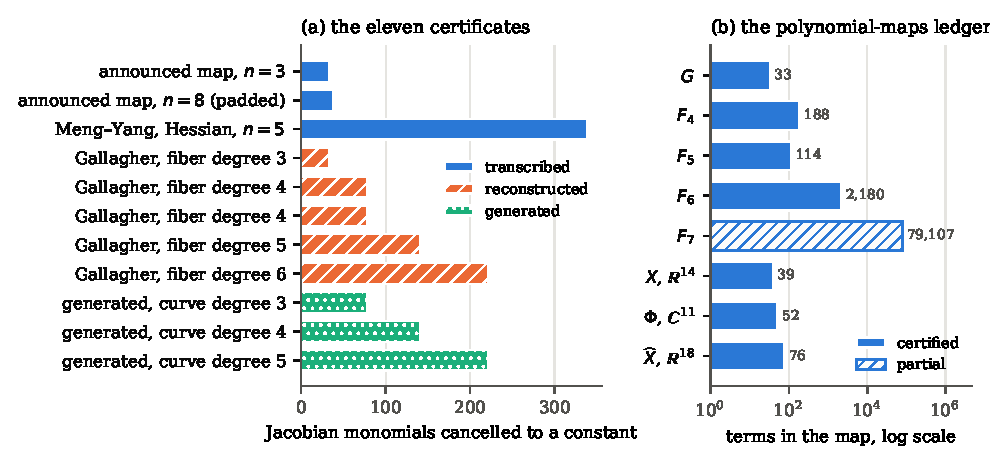
\includegraphics[width=\linewidth]{fig/jacobian-counterexamples-load.pdf}
\caption{The exact-arithmetic load of each decision, drawn from the records. (a)~For each
certificate of Record~I, the number of monomials in the symbolic Jacobian that the independent
verifier cancelled to a constant, grouped by lane. (b)~For each object of Record~II, the number
of terms in the map; $F_7$, hatched, is the one row decided in part.}\label{fig:load}
\end{figure}

\begin{theorem}[maps generated here]\label{thm:generated}
For the curves of degree \GenDegrees{} with coefficient vectors $[c_1,\dots,c_d]$ listed in
Table~\ref{tab:gen}, with $g_0=\GenGZero$ and $b=\GenB$, the tangent-sweep recipe yields three
polynomial maps $\C^3\to\C^3$, each with $\det J\equiv-2$ as a polynomial identity and two
distinct rational points sharing one image. By Lemma~\ref{lem:keller} each is a counterexample
to the Jacobian conjecture in dimension three. None of the three is printed in any of the pinned
sources.
\end{theorem}

\begin{proof}
The recipe's divisibility conditions are verified monomial by monomial and the three facts are
decided exactly as for a published claim; the certificate records the curve, the twist
coefficient $a$, the secant pair and the witnesses, and the verifier re-derives the determinant
from the monomial lists alone.
\end{proof}

\begin{table}[t]\centering\small
\resizebox{\linewidth}{!}{%
\begin{tabular}{llcclcl}\toprule
certificate & curve $[c_1,\dots,c_d]$ & $a$ & nominal geom.\ degree & component degrees & Jacobian monomials & the two witnesses\\\midrule
\GenRows
\bottomrule\end{tabular}}
\caption{The \NGenerated{} generated maps: new curves through the published mechanism, with
$g_0=\GenGZero$, $b=\GenB$ and $\det J\equiv-2$. The nominal geometric degree is $d+1$ by the
construction; what is decided is $\det J$ and the two witnesses, and for the first map a blind
count of at least three preimages (Table~\ref{tab:fib}, whose targets are these maps' images).}\label{tab:gen}
\end{table}

\begin{table}[t]\centering\small
\resizebox{\linewidth}{!}{%
\begin{tabular}{llcccl l}\toprule
certificate & seed $[c_1,\dots,c_d]$ & $a$ & $b$ & $\det J$ & nominal fiber degree & the two witnesses\\\midrule
\GalRows
\bottomrule\end{tabular}}
\caption{Gallagher's family rebuilt from its seeds under the paper's gauge ($c=1$ throughout;
$\det J=bc$). The seeds for $d=2,\dots,5$ are the paper's $p_d=2w-3w^2+w(1-w)(w^{d-2}-6/(d(d+1)))$,
and the last row is its distinct member $p=w-2w^3$ with $b=-1$, whose twist coefficient
$a=-\tfrac{4}{3}$ matches the paper.}\label{tab:gal}
\end{table}

A remark on what ``generated here'' means. A new curve through a published mechanism is a new
instance, not a new mechanism; the construction is Speyer's as written up by Gao, and this
repository claims none of it. The three maps have not been checked for coordinate equivalence
against the members of the published family (\S\ref{sec:moduli}). What is certified is what the
certificate says: these polynomials, this determinant, these two points.

\begin{proposition}[the doubling identity, recomputed]\label{prop:doubling}
Let $F$ be the announced map and $\varphi=y\cdot F=\sum_{i=1}^3y_iF_i$ in six variables
(\DoublingPhiMonos{} monomials). Then $\det\Hess\varphi\equiv\DoublingDet=-(\det J(F))^2$.
\end{proposition}

\begin{proof}
The $6\times6$ Hessian (\DoublingHessMonos{} monomials in total) is expanded symbolically at
every build and at the run that wrote this document; the constant is \DoublingDet. This is the
six-variable Hessian counterexample Meng--Yang record as a warm-up, and the identity is what ties
the two transcribed entries of Record~I to each other: the five-variable $\Psi$ descends from
$\varphi$ by a Schur complement, and if the transcription of either object were wrong the
recomputed constant would not be $-(\AlpogeDet)^2$. Both entries pin the same file, so this is an
arithmetic independence and not a second source.
\end{proof}

\section{Record I, continued: the collisions found blind}\label{sec:blind}

Everything in \S\ref{sec:cert} decides witnesses somebody supplied. This section supplies none.
For each three-dimensional map of Record~I and a rational target, the fiber counter of
\S\ref{sec:instrument} hunts preimages with \FibStarts{} Newton starts over a ladder of scales and
certifies every candidate it reaches in a Krawczyk box on the exact map.

\begin{theorem}[blind fiber counts]\label{thm:blind}
For each cell of Table~\ref{tab:fib} with verdict ``certified'', the map has at least the stated
number of preimages of the stated target, each in an explicit box in which it is the unique
preimage, the boxes pairwise disjoint. In particular the announced map has at least three
preimages of \AlpogeImage{} and at least three preimages of \OwnTarget, so it is not injective,
with no published witness consumed.
\end{theorem}

\begin{proof}
Krawczyk's criterion with strict interior containment on interval-enclosed exact coefficients
\cite{Krawczyk1969}; disjoint boxes hold distinct points. For the first cell each of the three
published witnesses lies inside one of the three certified boxes, which is the check that the
rediscovery is of the same points and not of three others; the hunt never read them. The target
\OwnTarget{} of the second cell was chosen here by a fixed enumeration of plain rational points,
$(0,0,0),(1,1,1),(1,0,0),(0,1,0),\dots$, the first whose blind count certifies at least two; it is
nobody's published image and nobody's constructed collision.
\end{proof}

\begin{table}[t]\centering\small
\resizebox{\linewidth}{!}{%
\begin{tabular}{llllccl}\toprule
cell & map & target & target from & witnesses constructed & certified blind & verdict\\\midrule
\FiberRows
\bottomrule\end{tabular}}
\caption{The fiber family, re-run at the run that wrote this document: \FibHits{} of \FibCells{}
cells certify non-injectivity blind. A count is a lower bound; a cell that returns one box
(\verdict{reject}) or none (\verdict{refused}) proves nothing and says so.}\label{tab:fib}
\end{table}

Three facts in the table deserve attention. In \FibExceeded{} cells (\FibExceededCells) the hunter
certifies more preimages than the two witnesses its own construction wrote down, consistent with
the nominal geometric degrees of those maps but proving only the lower bound. In two cells
(\FibFailedCells) the hunt does not certify non-injectivity at all: the float layer did not reach
enough roots, and the certificate reports one box or none rather than rounding up. Those maps are
still certified non-injective by Theorem~\ref{thm:published} and Theorem~\ref{thm:generated};
the counter simply did not re-find it unaided, and a lower bound that is allowed to be weak is
the only kind that can be trusted when it is strong. Finally, the control that makes the counts
mean something: a preimage counter that manufactured non-injectivity would find extra roots
everywhere, so it is run against the triangular automorphism $(x+y^2,\ y+z^3,\ z)$, injective by
construction with $\det J=1$; over \AutoStarts{} starts on the same ladder the dedup by certified
box disjointness returns exactly one preimage.

\section{Record II: Gao's five maps}\label{sec:gao}

Gao's paper \cite{Gao2026} (arXiv \GaoArxiv) prints $G$, $F_4$ and $F_5$ in full, and $F_6$ and
$F_7$ through their construction: four potentials, a direction field, a weighted scaling, a stage
map and a monomial substitution, with the first component printed and the term counts of the
others stated. The paper reports that \GaoAncillary{} (as recorded in the corpus metadata when
the sources were pinned). The verdicts on $F_6$ and $F_7$ are therefore
on the map the printed construction defines: the decider rebuilds each from the printed recipe,
checking every division exact, and checks the rebuild against every piece the paper does print
(the four printed polynomials $X_1,\dots,X_4$ and the first component for $F_6$; the first
component for $F_7$). The non-injectivity witnesses are found by this repository from each paper's
fiber structure, by a proposer the decider does not trust: it only evaluates them.

\begin{theorem}[Gao's maps, decided]\label{thm:gao}
Decided in exact rational arithmetic from the pinned TeX, at the ledger of \PolyGenerated{}:
\begin{enumerate}
\item $G\colon\C^3\to\C^3$ (\TermsG{} terms) has $\det J(G)\equiv2$ and two distinct rational
points with image \GaoImageG.
\item $F_4\colon\C^4\to\C^4$ (\TermsFfour{} terms) has $\det J(F_4)\equiv-\tfrac{44}{9}$ and
\FfourPoints{} distinct rational points with image \GaoImageFfour.
\item $F_5\colon\C^4\to\C^4$ (\TermsFfive{} terms) has $\det J(F_5)\equiv\tfrac{160}{29}$ and
two distinct rational points with image \GaoImageFfive.
\item $F_6\colon\C^5\to\C^5$, rebuilt from the printed construction with component degrees
\FsixDegs{} and \FsixTermsList{} terms (\TermsFsix{} in all), has $\det J(F_6)\equiv-290$ by
direct expansion of the $5\times5$ determinant, and two distinct rational points with image
\GaoImageFsix.
\end{enumerate}
By Lemma~\ref{lem:keller}, each is a counterexample to the Jacobian conjecture in its dimension.
The component degrees agree with the printed ones in every case.
\end{theorem}

\begin{proposition}[$F_7$, decided in part]\label{prop:f7}
The map $F_7\colon\C^5\to\C^5$ that the printed construction defines has component degrees
\FsevenDegs{} and \FsevenTermsList{} terms, reproduces the printed first component, and sends two
distinct rational points to one image, so it is not injective. The determinants of its factors
are as the paper states: $\det J(S)=\gamma$ for the sweep, $119377$ for the affine stage, and
$\det J_{(w_2,w_3)}(H_3,H_4)=1$ for the transverse data. The constancy of $\det J(F_7)$ itself is
not decided here.
\end{proposition}

\begin{proof}[Why it is partial]
The whole $5\times5$ determinant has rows of between \FsevenTermsMin{} and \FsevenTermsMax{}
terms, and its direct expansion is out of reach of the pure-Python decider in the time the ledger
allows; the constant rests on the paper's chain factorisation
$x^{10}\cdot119377\cdot\gamma^{8}\cdot\gamma^{2}\cdot(\gamma x)^{-10}$, whose factors are decided
and whose assembly is the paper's lemma. The ledger records the check with a null result, the
verdict \verdict{partial}, and the row names what would close it: a formalised chain rule for the
factorisation, or a determinant routine that expands rows of that size.
\end{proof}

\begin{table}[t]\centering\small
\resizebox{\linewidth}{!}{%
\begin{tabular}{lrlrclccl}\toprule
map & $n$ & component degrees & terms & $\det J$ & how decided & points & generic fiber (paper) & verdict\\\midrule
\GaoRows
\bottomrule\end{tabular}}
\caption{Gao's five maps. ``Terms'' counts all components; ``points'' is the number of distinct
rational points sharing one image; ``generic fiber'' is the paper's theorem statement, read
from the pinned TeX and not decided here. The whole ledger re-derives in about \PolySeconds{}
seconds.}\label{tab:gao}
\end{table}

The paper's generic fiber sizes (Table~\ref{tab:gao}, and \FiberAlpoge{} for the announced map)
are not decided in either record. Their proofs in \cite{Gao2026} run through univariate
elimination, squarefreeness and gcd certificates at witness targets; the instruments here
decide lower bounds only (Theorem~\ref{thm:blind}), and the exact counts are listed in
\S\ref{sec:not} as the first thing a next version should close.

\section{Record II, continued: the weak Markus--Yamabe fields}\label{sec:my}

The paper of Casta\~neda, Honorato and Valenzuela-Henr\'iquez \cite{CHV2026} (arXiv \ChvArxiv)
prints three objects: the field $X$ on $\mathbb{R}^{14}$ obtained from the announced map by the
chain realisation, the cubic map $\Phi$ on eleven variables that is the map's cubic stabilisation
in the sense of Bass--Connell--Wright, and the cubic field $\widehat X$ on $\mathbb{R}^{18}$
obtained from $\Phi$ by a rank-reduced dehomogenisation. The chain dimension is computed from the
announced map's component degrees as recorded in Record~I: $\sum_i\max(d_i,2)-n=\ChainSum-3=
\ChainN$, which is the dimension of the field the ledger decides.

\begin{theorem}[the fields, decided]\label{thm:my}
Decided in exact rational arithmetic from the pinned TeX, at the same ledger:
\begin{enumerate}
\item $X\colon\mathbb{R}^{14}\to\mathbb{R}^{14}$, of degree \XfourteenDeg{} with
\XfourteenTerms{} terms, satisfies $(JX+I)^{\XfourteenNil}=0$ identically (and no lower power
vanishes), and vanishes at the \XfourteenZeros{} distinct rational points the paper prints. By
Lemma~\ref{lem:my} the weak Markus--Yamabe conjecture is false in dimension $14$ and in every
dimension above it.
\item $\widehat X\colon\mathbb{R}^{18}\to\mathbb{R}^{18}$, of degree \XeighteenDeg{} with
\XeighteenTerms{} terms, satisfies $(J\widehat X+I)^{\XeighteenNil}=0$ identically (and no lower
power vanishes), and vanishes at \XeighteenZeros{} distinct rational points. The weak conjecture is
therefore also false in dimension $18$ by a field of degree three.
\item $\Phi\colon\C^{11}\to\C^{11}$, cubic with \PhiTerms{} terms, has $\det J(\Phi)\equiv-2$
by a direct $11\times11$ expansion, and \PhiPoints{} distinct points share one image; it is a cubic
counterexample to the Jacobian conjecture in dimension $11$.
\end{enumerate}
\end{theorem}

\begin{proof}
The matrix powers are multiplied out as matrices of exact polynomials; the zeros and images are
evaluated as fractions. For $\widehat X$ the pinned appendix checks the unipotency ``at a sample
rational point'' with a computer-algebra system; here the vanishing of the seventeenth power is
an identity, which is what Lemma~\ref{lem:my} needs at every point. For $\Phi$ the paper
verifies the determinant through a $3\times3$ Schur complement; the direct expansion decides
the same constant.
\end{proof}

\begin{table}[t]\centering\small
\begin{tabular}{lrrrlll}\toprule
object & $N$ & degree & terms & identity decided & zeros / points & verdict\\\midrule
\FieldRows
\bottomrule\end{tabular}
\caption{The three objects of \cite{CHV2026}, as decided. For $\Phi$ the identity is a constant
determinant and the points are three with one image; for the fields it is the nilpotency of
$JX+I$ as a matrix of polynomials, with the index that first vanishes.}\label{tab:fields}
\end{table}

A note on provenance, recorded in the corpus metadata rather than decided: \PhiProvenance{}
The certificate is indifferent to who wrote the map; the fact is recorded because the decision
grammar of this paper exists for exactly such objects.

\section{The moduli question, open}\label{sec:moduli}

The generator of \S\ref{sec:instrument} is a parametrised family. At curve degree $d$ the
coefficients $c_3,\dots,c_d$ are free, $c_1,c_2$ are determined by the two divisibility
conditions, and $g_0$ and $b$ are free nonzero constants; the three shipped instances take
$g_0=\GenGZero$, $b=\GenB$, $c_d=1$ and the remaining free coefficients zero. Gallagher's gauge
parametrises the same mechanism differently, and the paper's family realises every generic fiber
degree $d\ge3$ in dimension three. Composition with polynomial automorphisms on either side
identifies many of these maps, and, as \cite{Gao2026} notes, geometric degree is invariant under
such composition; beyond that invariant nothing is decided here, and no equivalence-testing
instrument exists in the repository.

\paragraph{Question.} For each geometric degree $k\ge3$, how many coordinate-inequivalent
Keller counterexamples $\C^3\to\C^3$ does the tangent-sweep family contain, and is every
dimension-three counterexample equivalent to one of them? The three generated maps of
Theorem~\ref{thm:generated} have nominal geometric degrees \GenGeomDegrees{}; whether the first
is equivalent to Gallagher's $d=3$ member or to the distinct member (both of nominal degree $4$),
or the second and third to the $d=4$ and $d=5$ members, is not known to us. The record labels
every generated row ``not coordinate-equivalence-checked'' for this reason.

\section{What is not claimed}\label{sec:not}

The certificates are narrow on purpose; the value of a narrow claim is that it is either true or
refuted. Stated plainly:
\begin{itemize}
\item \emph{Not that the external papers stand.} Each is cited as a claim and its bytes are
pinned. Whether it is correct as a paper, survives refereeing, or has been contested since the
pinned version is not decided here. Every verdict concerns the explicit object printed in the
record, and \verdict{partial} on $F_7$ measures this instrument's reach, not the paper.
\item \emph{No priority, in either direction.} Sources are recorded as transcribed, with the
dates they carry. The generated maps are new instances of a published mechanism.
\item \emph{Nothing about the plane.} Every map here has $n\ge3$; the two-dimensional case is
untouched, as is the Hessian conjecture in four variables.
\item \emph{One stabilisation, not six theorems.} Identity padding carries a counterexample to
every higher dimension unchanged; the record carries one padded row, at $n=\PaddedN$, whose
certificate text says it is padding.
\item \emph{Lower bounds only on fibers.} The blind counts are ``at least $k$''. The generic
fiber sizes of Gao's theorems (\FiberG, \FiberFfour, \FiberFfive, \FiberFsix, \FiberFseven{} and
\FiberAlpoge{} for the announced map) and the nominal geometric degrees of the generated and
rebuilt maps are not decided; they would need squarefreeness and gcd certificates at witness
targets together with certified boxes, which are not built.
\item \emph{$F_7$'s whole determinant.} Only its factors are decided (Proposition~\ref{prop:f7}).
\item \emph{The chain cannot be shortened.} The Markus--Yamabe paper states that moving any
homogeneous part one level up destroys the nilpotency and that this was verified in exact
arithmetic; it prints no certificate, and the finite family of variants is not decided here.
\item \emph{Nothing beyond the identities for the dynamics.} Hyperbolic sinks, almost global
stability and the discrete counterpart in \cite{CHV2026} are consequences the paper draws from the
spectrum; only the spectrum, as the nilpotency identity, and the zeros are decided.
\item \emph{No proof by a language model.} Models are in no decision path. The instrument, the
generator, the fiber counter, the batteries and the verifier are deterministic code, and every
verdict is a finite exact computation a reader can re-run.
\end{itemize}

\cmrepro{Record~I: \texttt{certs/keller-certificate.json} (the \NCerts{} certificates, every
polynomial as explicit monomials with exact rational coefficients), written by
\texttt{tools/export-keller-certificate.js} from \texttt{families/keller-audit.js};
\texttt{python3 tools/verify\_keller.py certs/keller-certificate.json --sources corpus/sources}
re-decides all \NCerts{} in a fraction of a second with the standard library only and must refute a
forged coefficient before exiting green; \texttt{node instruments/keller/battery.js} runs the
instrument's gate (\BatPass{} checks, \BatReds{} red controls, the generator calibration and the
blind rediscovery); \texttt{node tools/build-report-keller.js} rebuilds the public page
\url{https://carlostoledo.co/reports/keller.html}, re-running every gate, the fiber family
(\texttt{families/keller-fibers.js}, about ten seconds) and the doubling identity. The instrument
is \texttt{instruments/keller/} (\texttt{keller.js} the audit, \texttt{sweep.js} the generator and
Gallagher's gauge, \texttt{fibers.js} the Krawczyk fiber counter). Sources pinned in
\texttt{corpus/sources/}: \PinFiles{} (hashes in \texttt{PINS.json} and in the certificate).
Record~II: \texttt{certs/polymaps-ledger.json}, written by \texttt{tools/run-polymaps-ledger.py}
from \texttt{instruments/polymaps/decide.py} over \texttt{corpus/polymaps/} (the two TeX sources
under CC~BY~4.0, \texttt{maps.json} extracted by \texttt{extract.py}, the witnesses in
\texttt{witnesses.json}); \texttt{python3 tools/run-polymaps-ledger.py --check} re-derives it in
about \PolySeconds{} seconds and refuses on any difference; \texttt{python3
instruments/polymaps/battery.py} runs its gate; the page is
\url{https://carlostoledo.co/reports/polymaps.html}. This document: \texttt{node
tools/paper-numbers/jacobian-counterexamples.js} writes every macro from the two records and the
live runs (git \RepoCommit), \texttt{tools/paper-numbers/jacobian-counterexamples-fig.py} draws
Figure~\ref{fig:load}, and \texttt{node tools/build-paper-tex.js jacobian-counterexamples}
compiles. The repository is archived under concept DOI
\href{https://doi.org/10.5281/zenodo.22225860}{10.5281/zenodo.22225860}.}

\begin{thebibliography}{99}\small
\bibitem{Keller1939} O.-H.~Keller, Ganze Cremona-Transformationen, Monatsh.\ Math.\ Phys.\ 47 (1939), 299--306.
\bibitem{BCW1982} H.~Bass, E.~H.~Connell, D.~Wright, The Jacobian conjecture: reduction of degree and formal expansion of the inverse, Bull.\ Amer.\ Math.\ Soc.\ (N.S.) 7 (1982), 287--330.
\bibitem{Essen2000} A.~van den Essen, Polynomial Automorphisms and the Jacobian Conjecture, Progress in Mathematics 190, Birkh\"auser, Basel, 2000.
\bibitem{Wang1980} S.~S.-S.~Wang, A Jacobian criterion for separability, J.\ Algebra 65 (1980), 453--494.
\bibitem{Moh1983} T.-T.~Moh, On the Jacobian conjecture and the configurations of roots, J.\ Reine Angew.\ Math.\ 340 (1983), 140--212.
\bibitem{BBR1962} A.~Bia{\l}ynicki-Birula, M.~Rosenlicht, Injective morphisms of real algebraic varieties, Proc.\ Amer.\ Math.\ Soc.\ 13 (1962), 200--203.
\bibitem{dBE2005} M.~de Bondt, A.~van den Essen, A reduction of the Jacobian conjecture to the symmetric case, Proc.\ Amer.\ Math.\ Soc.\ 133 (2005), 2201--2205.
\bibitem{Alpoge2026} L.~Alp\"oge, announcement of an explicit counterexample to the Jacobian conjecture in dimension three, 19 July 2026, \url{https://x.com/__alpoge__/status/2079028340955197566}; the map and its three witnesses are printed as eq.\ (1)--(2) of \cite{MengYang2026}, the bytes this record pins.
\bibitem{Gallagher2026} A.~Gallagher, An infinite family of counterexamples to the Jacobian Conjecture in dimension three: every generic fiber degree $n\ge3$ occurs, preprint, 20 July 2026, Zenodo, \href{https://doi.org/10.5281/zenodo.21479195}{doi:10.5281/zenodo.21479195}.
\bibitem{Tao2026} T.~Tao, A digestion of the Jacobian conjecture counterexample, blog post, 21 July 2026, \url{https://terrytao.wordpress.com/2026/07/21/a-digestion-of-the-jacobian-conjecture-counterexample/} (as recorded in the bibliography of \cite{Gao2026}).
\bibitem{Speyer2026} D.~E.~Speyer, The geometry and structure of Gallagher's counterexamples to the Jacobian conjecture, note, 23 July 2026, \url{https://sbseminar.wordpress.com/wp-content/uploads/2026/07/jacobiantangentsweep.pdf} (as recorded in the bibliography of \cite{Gao2026}).
\bibitem{MengYang2026} G.~Meng, L.~Yang, A five-variable counterexample to the Hessian conjecture, and the low-dimensional status of the Jacobian and Hessian conjectures, arXiv:2607.22198v2 [math.AC], 27 July 2026.
\bibitem{Gao2026} S.~Gao, \GaoTitle, arXiv:\GaoArxiv{} [math.AG], August 2026.
\bibitem{CHV2026} \'A.~Casta\~neda, G.~Honorato, F.~Valenzuela-Henr\'iquez, \ChvTitle, arXiv:\ChvArxiv, August 2026.
\bibitem{MarkusYamabe1960} L.~Markus, H.~Yamabe, Global stability criteria for differential systems, Osaka Math.\ J.\ 12 (1960), 305--317.
\bibitem{Fessler1995} R.~Fe\ss ler, A proof of the two-dimensional Markus--Yamabe stability conjecture and a generalization, Ann.\ Polon.\ Math.\ 62 (1995), 45--74.
\bibitem{Gutierrez1995} C.~Guti\'errez, A solution to the bidimensional global asymptotic stability conjecture, Ann.\ Inst.\ H.\ Poincar\'e Anal.\ Non Lin\'eaire 12 (1995), 627--671.
\bibitem{Cima1997} A.~Cima, A.~van den Essen, A.~Gasull, E.~Hubbers, F.~Ma\~nosas, A polynomial counterexample to the Markus--Yamabe conjecture, Adv.\ Math.\ 131 (1997), 453--457.
\bibitem{AFP2026} A.~Freitas Ramos, D.~Barros Hulak, R.~J.~G.~B.~de Queiroz, Formal verification of an explicit counterexample to the Jacobian conjecture, Archive of Formal Proofs, 2026, \url{https://isa-afp.org/entries/Jacobian_Counterexample.html} (as recorded in the bibliography of \cite{CHV2026}; not consulted here).
\bibitem{Spacerat2026} Spacerat, 11 variable cubic Jacobian conjecture counterexample, GitHub Gist, July 2026, \url{https://gist.github.com/Spacerat/08b4a43f6b6ca57178efabc220170ce8}; its map was compared term for term with $\Phi$ when the corpus was pinned.
\bibitem{Krawczyk1969} R.~Krawczyk, Newton-Algorithmen zur Bestimmung von Nullstellen mit Fehlerschranken, Computing 4 (1969), 187--201.
\end{thebibliography}

\end{document}
